% ============================================================
% KG Discovery Engine — Paper Manuscript
% Alignment-Driven Cross-Domain Hypothesis Generation in Knowledge Graphs
%
% Compile: pdflatex main.tex
% Required packages: graphicx, booktabs, hyperref, amsmath, microtype,
%                    geometry, enumitem, xcolor, tabularx
% ============================================================
\documentclass[11pt,a4paper]{article}

% Core packages
\usepackage[margin=1in]{geometry}
\usepackage{graphicx}
\usepackage{booktabs}
\usepackage{hyperref}
\usepackage{amsmath}
\usepackage{amssymb}
\usepackage{microtype}
\usepackage{enumitem}
\usepackage{xcolor}
\usepackage{tabularx}
\usepackage{multirow}
\usepackage{url}
\usepackage{natbib}

% Hyperref setup
\hypersetup{
  colorlinks=true,
  linkcolor=blue!70!black,
  citecolor=green!50!black,
  urlcolor=blue!70!black,
}

% Figure path
\graphicspath{{figures/}}

% ============================================================
% Title and authors
% ============================================================
\title{Alignment-Driven Cross-Domain Hypothesis Generation\\
       in Knowledge Graphs}

\author{[Author Placeholder]\\
        [Institution Placeholder]\\
        \texttt{[email@placeholder.example]}}

\date{\today}

% ============================================================
\begin{document}

\maketitle

% ------ Abstract ------
\begin{abstract}
Cross-domain hypothesis generation---discovering mechanistic links between two
domain-specific knowledge graphs---requires traversing graph boundaries that no
single-domain operator can cross.
We present a multi-operator pipeline consisting of \textit{align}, \textit{union},
\textit{compose}, \textit{difference}, and \textit{evaluate} operators, and study its
behaviour on Wikidata-derived bio-chem knowledge graph pairs across three independent
domain contexts (cancer signaling, immunology, and neuroscience).

Our experiments establish three findings.
(1)~The \textit{align} operator is necessary and sufficient to unlock
alignment-dependent cross-domain paths: without it, the compose operator produces
zero cross-domain candidates; with it, the pipeline generates dozens to hundreds of
structurally unique cross-domain path candidates, scaling non-linearly with graph size.
(2)~Raw multi-hop output from real knowledge graphs contains substantial semantic
drift---25\% of deep candidates are structurally non-mechanistic---and a relation-type
filter derived from qualitative review reduces drift to 0\% while preserving all
scientifically meaningful candidates, generalising across all three domain pairs
without parameter retuning.
(3)~The number of unique cross-domain candidates is better predicted by the structural
diversity of bridge entities than by their count: neurotransmitter and eicosanoid bridges
yield 6--8$\times$ more candidates per bridge pair than a single-metabolite bridge.

We further identify a fundamental limitation of the current pipeline: the knowledge
graph encodes relation types at the class level rather than the instance level,
which means filter-passing candidates can carry chemically invalid edges that the
filter cannot detect without substrate-specificity metadata.
This finding, from a post-hoc relation semantics audit (Run~014),
constrains all candidate interpretations and is the central theme of
the Limitations and Discussion sections.
Code and all experimental artefacts will be released upon acceptance
(repository link provided in the supplementary material).
\end{abstract}


% ------ 1. Introduction ------
\section{Introduction}
\label{sec:intro}

Scientific discovery increasingly occurs at disciplinary boundaries.
The mechanisms by which a gene mutation in cancer signaling alters metabolic chemistry,
or how a neurotransmitter synthesis enzyme predicts pharmacological drug sensitivity,
are precisely the cross-domain questions that no single-domain knowledge graph (KG)
can answer in isolation.

Existing approaches to KG-based discovery---link prediction~\cite{TODO-TransE,TODO-RotatE},
KG completion~\cite{TODO-ComplEx}, and semantic similarity methods---operate within
a single KG schema.
They can predict missing edges within a domain but cannot generate hypotheses that
cross the boundary between two independently curated domain graphs with disjoint
node vocabularies.

We address this gap with a multi-operator pipeline that treats cross-domain discovery
as a graph composition problem.
The key operator is \textbf{align}: it identifies bridge entities shared between two
domain KGs (e.g., a metabolite that appears in both a biological signaling graph and
a chemical reaction graph under different identifiers), collapses them into shared
nodes, and enables the \textbf{compose} operator to enumerate multi-hop paths that
cross the domain boundary.
Without alignment, compose produces zero cross-domain candidates; with alignment,
it produces structurally unique paths connecting biological genes and proteins
to chemical reaction classes and functional groups.

The pipeline builds on Swanson's ABC discovery model~\cite{swanson1986fish}, which
finds implicit connections $A \to C$ via a shared concept $B$ in two literatures.
Our contribution is to formalise this as a graph-algebraic operator pipeline,
to study its empirical behaviour on real Wikidata-derived knowledge graphs, and to
characterise the conditions under which its output is scientifically meaningful.

\subsection*{Contributions}

This paper makes three empirical contributions:

\begin{enumerate}[leftmargin=*, label=\textbf{\arabic*.}]

\item \textbf{Alignment is necessary for cross-domain reachability.}
Without bridge alignment, the compose operator produces zero cross-domain
candidate pairs.
With alignment, it produces 5--55 alignment-dependent unique cross-domain paths
per domain pair, scaling non-linearly with KG size.
Replicated across 3 independent bio-chem domain pairs.

\item \textbf{Quality filtering makes raw deep output useful.}
Raw 3-hop+ cross-domain candidates from real KGs contain
25\% semantically drifted content (structural-chemical expansions
rather than mechanistic hypotheses).
A relation-type filter derived from qualitative review of one domain pair
eliminates all drift while preserving all promising candidates, and
transfers across two independent domain pairs without parameter adjustment.

\item \textbf{Bridge structural diversity, not bridge count, drives candidate yield.}
Across three domain pairs with 5--9 aligned bridge pairs,
unique-to-alignment candidate counts vary from 5 to 55.
This variation is explained by bridge entity dispersion (the number of
distinct downstream nodes each bridge class connects to), not by bridge count.

\end{enumerate}

We also contribute a negative finding: a post-hoc relation semantics audit
reveals that all five qualitatively reviewed candidates carry at least one
relation edge where the class-level KG encoding cannot validate
substrate-specific chemical or biological claims.
This finding unifies previously separate candidate weaknesses under a single
root cause and is the primary open problem for future work.

The remainder of this paper is structured as follows.
Section~\ref{sec:related} reviews related work.
Section~\ref{sec:method} describes the pipeline operators and scoring rubric.
Section~\ref{sec:setup} presents the experimental setup and data.
Section~\ref{sec:results} reports the main results for Claims 1--3.
Section~\ref{sec:casestudies} presents five representative candidate case studies.
Section~\ref{sec:discussion} interprets the findings, with relation semantic
insufficiency as the central theme.
Sections~\ref{sec:threats}--\ref{sec:limitations} address threats to validity
and limitations.
Section~\ref{sec:conclusion} concludes with future work priorities.


% ------ 2. Related Work ------
\section{Related Work}
\label{sec:related}

\subsection{KG Completion and Link Prediction}

Methods such as TransE~\cite{TODO-TransE}, RotatE~\cite{TODO-RotatE}, and
ComplEx~\cite{TODO-ComplEx} learn entity and relation embeddings to predict missing
edges within a single KG.
These approaches assume a shared schema and are designed to densify an existing graph,
not to generate hypotheses that cross between two graphs with disjoint schemas.
Multi-relational embedding approaches similarly operate within a unified ontological
space and cannot represent the structural boundary between two independently curated
domain knowledge graphs.

\subsection{Multi-KG Alignment}

Entity alignment~\cite{TODO-entity-alignment-survey},
schema alignment~\cite{TODO-schema-alignment}, and ontology
matching~\cite{TODO-ontology-matching} address the problem of mapping entities
between knowledge graphs.
These methods focus on constructing the mapping itself, not on exploiting it to
generate cross-domain hypothesis candidates.
Our \textit{align} operator draws on this literature but is operationalised
specifically to enable path-based cross-domain traversal via the subsequent
\textit{union} and \textit{compose} steps.

\subsection{Biomedical KG Discovery}

SemMedDB~\cite{TODO-SemMedDB} and drug repurposing systems such as
PREDICT~\cite{TODO-PREDICT} use predicate-level associations mined from the
biomedical literature for mechanism discovery and drug repurposing.
These systems operate within a unified biomedical ontology (a single-schema KG)
rather than across two independently curated domain graphs.
Production-scale biomedical KGs such as Hetionet~\cite{TODO-Hetionet} and
PrimeKG~\cite{TODO-PrimeKG} represent a single integrated schema and therefore
do not exhibit the structural cross-domain boundary we study.
Our work is complementary: it studies the behaviour of a multi-operator pipeline
on small-to-medium Wikidata-derived KGs, with the goal of characterising the
structural conditions for cross-domain discovery.

\subsection{Operator-Based KG Reasoning}

Description logics~\cite{TODO-description-logics} and rule-based
reasoners~\cite{TODO-rule-reasoning} derive implicit facts within a schema but
do not define operators for cross-KG path composition.
Our work introduces a graph-algebraic operator vocabulary (align, union, compose,
difference, evaluate) as the compositional primitive for cross-domain discovery.

\subsection{Swanson's ABC Model and Literature-Based Discovery}

The classic ABC discovery model~\cite{swanson1986fish} finds implicit connections
$A \to C$ in two separate literatures via a shared intermediate concept $B$.
The seminal example is the fish-oil / migraine / Raynaud's syndrome connection:
literature~1 linked $A$ (fish oil) to $B$ (blood rheology), while literature~2
linked $B$ (blood rheology) to $C$ (Raynaud's syndrome), yet the connection
$A \to C$ was not explicitly stated in either.
Our \textit{align} operator implements a structural analogue: bridge entities $B$
shared between $G_{\text{bio}}$ and $G_{\text{chem}}$ enable $A \to B \to C$
paths that cross the domain boundary.
Our contribution is to formalise this as a KG operator pipeline, to characterise
the conditions under which the mechanism produces useful output, and to identify
the principal source of semantic failures in the generated candidates.


% ------ 3. Method ------
\section{Method}
\label{sec:method}

\begin{figure}[t]
  \centering
  \includegraphics[width=0.92\linewidth]{figures/figure1_pipeline.png}
  \caption{%
    \textbf{Pipeline overview.}
    Two domain-specific KGs ($G_{\text{bio}}$, $G_{\text{chem}}$) with disjoint
    node sets are combined through five operators.
    The \textit{align} step identifies bridge entities shared between domains and
    creates an alignment map; \textit{union} collapses aligned pairs into single
    bridge nodes in the merged graph $G_{\text{merged}}$.
    The \textit{compose} step performs BFS up to depth~5 with an optional drift
    filter, producing raw hypothesis candidates $H_{\text{raw}}$.
    The \textit{difference} step isolates domain-unique candidates;
    \textit{evaluate} scores each candidate on five dimensions.
    Without \textit{align}, compose produces zero cross-domain paths.
  }
  \label{fig:pipeline}
\end{figure}

\subsection{Knowledge Graph Representation}

A knowledge graph $G = (V, E, D)$ consists of:
\begin{itemize}[noitemsep]
  \item $V$: nodes with attributes (\textit{id}, \textit{label}, \textit{domain}
    $\in \{\text{bio}, \text{chem}\}$)
  \item $E$: directed edges with triples (\textit{source}, \textit{relation},
    \textit{target})
  \item $D$: domain attribute partitioning nodes into their origin KG
\end{itemize}

A \textit{HypothesisCandidate} is a path through the merged graph encoded as
an alternating sequence of node identifiers and relation labels, with full provenance.

\subsection{Pipeline Operators}

\paragraph{align($G_{\text{bio}}$, $G_{\text{chem}}$, $\theta$) $\to$ AlignmentMap.}
Returns a bijective mapping from $G_{\text{bio}}$ node IDs to $G_{\text{chem}}$ node
IDs where label similarity $\geq \theta$ (default 0.5).
Label similarity uses synonym-aware Jaccard tokenisation with a fixed synonym dictionary:
\{\textit{enzyme}$\leftrightarrow$\textit{catalyst},
  \textit{protein}$\leftrightarrow$\textit{compound},
  \textit{inhibit}$\leftrightarrow$\textit{block},
  \textit{reaction}$\leftrightarrow$\textit{process}\}.
In Phase~4 (Runs~007--013), known bridge metabolites (NADH, arachidonic acid,
neurotransmitters) are injected as pre-labelled hard alignment pairs, bypassing the
similarity step.

\paragraph{union($G_{\text{bio}}$, $G_{\text{chem}}$, alignment) $\to G_{\text{merged}}$.}
Merges both graphs, collapsing aligned pairs into single bridge nodes.
Unaligned nodes are namespace-prefixed to prevent ID collision.
After union, BFS can traverse from a bio node through an aligned bridge node
into the chem subgraph---the structural mechanism underlying all cross-domain
paths in this work.

\paragraph{compose($G_{\text{merged}}$, max\_depth, filter\_spec) $\to H_{\text{raw}}$.}
BFS from all source nodes to depth \texttt{max\_depth}$=5$.
Each reachable path becomes a \textit{HypothesisCandidate} with full provenance.
The drift filter (Section~\ref{sec:filter}) is applied within BFS.

\paragraph{difference($G_1$, $G_2$, alignment) $\to G_{\text{unique}}$.}
Returns $G_1$ nodes not covered by the alignment, used to enumerate domain-unique
candidate pairs (the \textit{unique\_to\_alignment} metric).

\paragraph{evaluate($H$, $G$, rubric) $\to H_{\text{scored}}$.}
Scores each candidate on five dimensions (Section~\ref{sec:rubric}).

\subsection{Drift Filter}
\label{sec:filter}

Derived from qualitative review of Subset~A candidates (Run~011),
the filter excludes four structural relation types and applies two path-level guards:

\begin{verbatim}
blocked:  {contains, is_product_of, is_reverse_of, is_isomer_of}
min_strong_ratio: 0.40
consecutive_repeat_guard: True
generic_intermediate_guard: True
\end{verbatim}

\noindent A path is rejected if:
(1)~any relation $\in$ \texttt{blocked} (structural-chemical expansions);
(2)~$\frac{|\text{strong relations}|}{|\text{all relations}|} < 0.40$, where
strong relations are \{inhibits, activates, catalyzes, produces, encodes,
accelerates, yields, facilitates\};
(3)~any relation type repeats consecutively;
(4)~any intermediate node label is in \{process, system, entity, substance, compound\}.

\subsection{Scoring Rubric}
\label{sec:rubric}

Each candidate is scored as:
\begin{equation}
  s = 0.30\,p + 0.25\,n + 0.20\,t + 0.15\,r + 0.10\,e
  \label{eq:score}
\end{equation}
where $p$=plausibility, $n$=novelty, $t$=testability, $r$=traceability, $e$=evidence support.

The traceability dimension was revised in Run~010: the original scorer penalised
long paths with $1/(d+1)$, making provenance-aware ranking equivalent to naive
depth ranking.
The revised scorer penalises low-specificity relations and generic intermediate
nodes regardless of path length (Table~\ref{tab:hypothesis_status}, H4 row).

\subsection{Path Interpretation Framework}
\label{sec:interpretation}

Run~014 introduced a post-hoc classification of all KG relation types by
inferential trustworthiness (Table~\ref{tab:relation_semantics}).
Five categories determine the maximum claim type that a composed path supports:

\begin{itemize}[noitemsep]
  \item \textbf{DM} (directional-mechanistic): safe for causal chaining
    (\textit{inhibits}, \textit{activates}, \textit{catalyzes}, \textit{encodes},
    \textit{produces}$_{\text{bio}}$)
  \item \textbf{DN} (directional-but-non-causal): ordering only, not mechanistic
    (\textit{undergoes}, \textit{is\_substrate\_of}, \textit{is\_precursor\_of})
  \item \textbf{SS} (symmetric-structural): structural fact, no causal direction
    (\textit{contains}, \textit{is\_isomer\_of}, \textit{is\_reverse\_of})
  \item \textbf{CD} (context-dependent): requires context annotation
    (\textit{reacts\_with})
  \item \textbf{CR} (chemically-risky): class-level generalisation requiring
    substrate-specificity pre-check
    (\textit{produces}$_{\text{rxn} \to \text{fg}}$)
\end{itemize}

The inferential power of a composed path is bounded by its weakest relation
category.
A path containing a CR relation cannot be treated as a mechanistic hypothesis
until the class-level generalisation is verified for the specific substrate.


% ------ 4. Experimental Setup ------
\section{Experimental Setup}
\label{sec:setup}

\subsection{Data: Wikidata-Derived Knowledge Graphs}

Three independent domain pairs were constructed from Wikidata SPARQL queries
with semi-manual bridge entity selection (Threat~T2.1; Section~\ref{sec:threats}).

\begin{description}[leftmargin=0pt]
\item[Subset~A --- Cancer Signaling / Metabolic Chemistry]
Bio KG: 293 nodes, 233 edges (cancer signaling genes, proteins, metabolites;
key entities: VHL, HIF1A, LDHA, NADH, mTOR, EGFR, KRAS).
Chem KG: 243 nodes, 191 edges (metabolic reactions and cofactors).
Aligned bridge pairs: 7 (NADH, NAD$^+$, ATP, ADP, Glucose, Pyruvate, Lactate).

\item[Subset~B --- Immunology / Natural Products]
Bio KG: 178 nodes, 122 edges (immune signaling, cytokines, receptors).
Chem KG: 110 nodes, 90 edges (natural products chemistry).
Aligned bridge pairs: 5 (eicosanoid metabolites: AA, PGE$_2$, LTB$_4$, PGI$_2$, TXA$_2$).

\item[Subset~C --- Neuroscience / Neuro-pharmacology]
Bio KG: 151 nodes, 128 edges (neurotransmitter synthesis, signaling).
Chem KG: 86 nodes, 78 edges (neuro-pharmacology, drug-receptor interactions).
Aligned bridge pairs: 9 (Dopamine, Serotonin, GABA, Norepinephrine + additional).
\end{description}

All experiments are fully deterministic (\texttt{random.seed=42}; no external API calls).

\subsection{Pipeline Conditions}

\begin{center}
\begin{tabular}{lll}
\toprule
Condition & Operators & Description \\
\midrule
P1 (single-op baseline) & compose only        & C1 condition; no alignment \\
P4 (multi-op)           & align+union+compose+difference+evaluate & C2; full pipeline \\
P4+filter               & P4 with drift filter & Run~012+ (Section~\ref{sec:filter}) \\
\bottomrule
\end{tabular}
\end{center}

\subsection{Evaluation Metrics}

\begin{itemize}[noitemsep]
  \item \textbf{unique\_to\_alignment}: cross-domain candidate pairs reachable
    only via aligned bridge nodes (zero in P1)
  \item \textbf{deep CD count}: candidates with path length $\geq 3$ and
    cross-domain subject/object
  \item \textbf{drift rate by depth}: fraction of candidates at each depth
    containing at least one blocked relation
  \item \textbf{promising rate}: fraction of deep CD candidates labelled
    \textit{promising} in qualitative review (Run~011; Subset~A only)
  \item \textbf{top-20 depth composition}: depth distribution of top-20 scored candidates
\end{itemize}

\subsection{Run Progression}
\label{sec:runs}

Thirteen runs span four phases: synthetic KG validation (Runs~001--006),
first real-data test (Run~007), scale-up and operator development
(Runs~008--012), and reproducibility testing (Run~013).
Table~\ref{tab:run_summary} summarises the key results at each phase.

\begin{table}[h]
\caption{%
  \textbf{Run progression summary (Runs 001--013).}
  Phase 1--2: synthetic KG; Phase 3--4: Wikidata-derived KGs.
  H1''/H3''/H4 verdicts reflect final hypothesis formulations (see text).
}
\label{tab:run_summary}
\small
\begin{tabularx}{\linewidth}{lcllX}
\toprule
Run & Phase & Scale & Key finding & Verdict \\
\midrule
001--006 & 1--2 & 57n (synth) & Operator validation, rubric calibration & H1/H3/H4 PASS (synthetic) \\
007      & 3    & 57n (real)   & H1'' cond.\ PASS; 4 unique pairs via alignment & H1'' PASS (cond.) \\
008      & 3    & 57n (real)   & H3'' FAIL: 57 nodes structurally incapable of 3-hop CD & H3'' FAIL (scale) \\
009      & 4    & 536n (real)  & H3'' PASS (20 deep CD); H4 FAIL (old rubric) & H1'',H3'' PASS; H4 FAIL \\
010      & 4    & 536n         & H4 PASS: revised traceability; 309 deep promoted & H4 PASS \\
011      & 4    & 536n         & Qualitative review: 25\% drift, 15\% promising & Manual labels \\
012      & 4    & 536n         & Drift filter: 0\% drift, 100\% promising; 3 survivors & Filter derived \\
013      & 4    & 288--536n    & Reproducibility 3/3 subsets SUCCESS & H1'',H3'' confirmed \\
\bottomrule
\end{tabularx}
\end{table}

\subsection{Hypothesis Definitions}

\begin{description}[leftmargin=0pt]
\item[H1'']
The multi-operator pipeline produces a non-zero number of
\textit{unique\_to\_alignment} cross-domain candidate pairs, demonstrating that
alignment-dependent paths exist that compose cannot reach without bridge alignment.

\item[H2]
The pipeline output is noise-robust under random edge deletion.
\textit{(Validated on synthetic KG only; not retested on real data.)}

\item[H3'']
On a real KG of sufficient scale ($\geq$288 nodes), the pipeline generates
$\geq$1 deep ($\geq$3-hop) cross-domain candidate that passes the drift filter
and is labelled promising (or inferred promising via filter passage).

\item[H4]
The revised quality-aware traceability scorer ranks deep cross-domain candidates
higher relative to the naive depth-penalty scorer.

\end{description}

Final hypothesis verdicts are reported in Table~\ref{tab:hypothesis_status}.


% ------ 5. Results ------
\section{Results}
\label{sec:results}

% Table 1: Hypothesis Status
% Source: paper_assets/final_metrics.json + docs/paper_claims.md
\begin{table}[h]
\caption{%
  \textbf{Final hypothesis verdicts (Runs~001--013).}
  H1'' and H3'' are the refined real-data hypotheses replacing the original
  synthetic-KG formulations.
  H2 was validated on synthetic KGs only and not retested on real data.
  H4 required rubric revision (Run~010) before passing.
  Confidence reflects replication count and evidence strength.
}
\label{tab:hypothesis_status}
\small
\begin{tabularx}{\linewidth}{llllX}
\toprule
Hypothesis & Verdict & Confidence & Evidence Runs & Notes \\
\midrule
H1'' & PASS & Very High &
  007, 009, 013A, 013B, 013C &
  Replicated 3/3 domain pairs; unique\_to\_alignment $>$0 in all cases \\
\addlinespace
H2  & Partial & Low &
  001--006 &
  Validated on synthetic KG only (50\% edge deletion);
  not retested on real data \\
\addlinespace
H3'' & PASS & High &
  009, 011, 012, 013A, 013B, 013C &
  Replicated 3/3 domain pairs;
  100\% promising rate after filter in all subsets \\
\addlinespace
H4  & PASS & High &
  009, 010 &
  Revised traceability scorer only;
  top-20 still 2-hop dominated in all configurations \\
\bottomrule
\end{tabularx}
\end{table}


\subsection{Claim 1: Alignment Unlocks Otherwise Unreachable Cross-Domain Paths}
\label{sec:result-c1}

\begin{figure}[t]
  \centering
  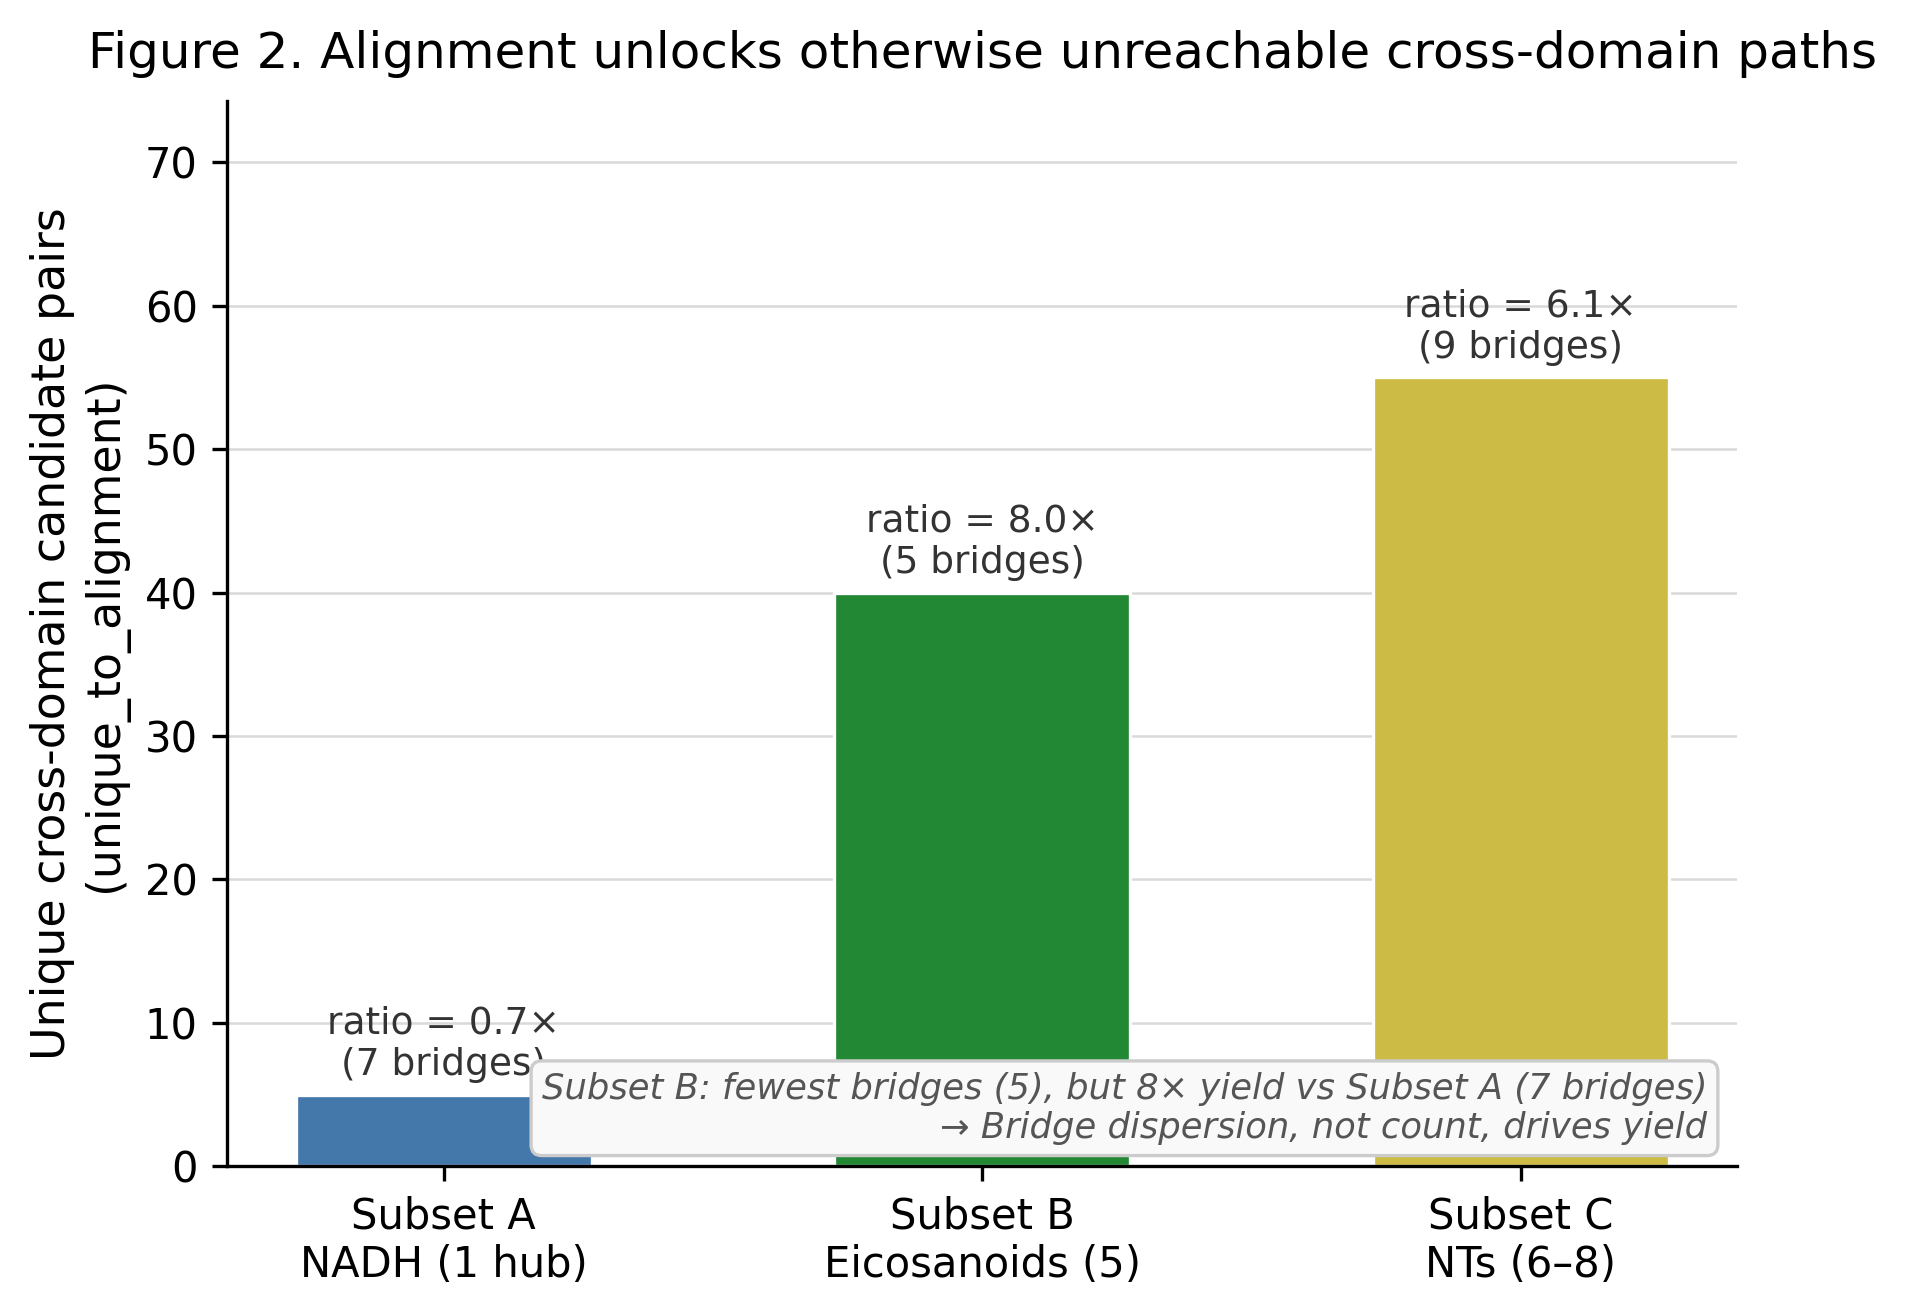
\includegraphics[width=0.88\linewidth]{figures/figure2_alignment_leverage.png}
  \caption{%
    \textbf{Alignment leverage across three domain pairs (Claim 1).}
    Each pair of bars shows total candidates and unique-to-alignment candidates
    for each subset.
    Without alignment (P1 baseline), unique-to-alignment candidates are always zero.
    Bridge count does not predict unique candidate yield: Subset~B (5 bridges) yields
    40 unique pairs while Subset~A (7 bridges) yields only 5, owing to differences in
    bridge structural diversity (Claim 3).
    Error bars not applicable (deterministic runs).
  }
  \label{fig:alignment_leverage}
\end{figure}

Without bridge alignment (P1), the compose operator produces zero cross-domain
candidate pairs across all tested configurations and scales.
With alignment (P4), the pipeline yields between 5 and 55 unique-to-alignment
cross-domain candidates depending on domain pair (Figure~\ref{fig:alignment_leverage}).

Scale amplification is non-linear: a 9$\times$ node increase (57$\to$536 nodes)
with 1.75$\times$ more bridges produces 42$\times$ more unique pairs (4$\to$168).
This is consistent with the theoretical expectation that BFS reachability
through bridge nodes grows with the product of bridge fan-out in both domains.

Run~013 confirms H1'' across all three independent domain pairs
(Table~\ref{tab:subset_comparison}): unique-to-alignment counts are
5 (Subset~A), 40 (Subset~B), and 55 (Subset~C).
The success criterion ($> 0$) is met in 3/3 subsets (confidence: very high).

% Table 2: Subset Comparison
% Source: paper_assets/subset_summary_table.csv
\begin{table}[h]
\caption{%
  \textbf{Subset comparison across three independent domain pairs (Run~013).}
  All three subsets achieve 0\% drift-heavy and 100\% promising rate after
  applying the filter derived from Subset~A without parameter retuning.
  Bridge class diversity, not bridge count, predicts unique candidate yield
  (unique/bridge ratios: 0.7, 8.0, 6.1 for A, B, C respectively).
  Drift-by-depth columns show fraction of candidates at each depth containing
  at least one blocked relation.
}
\label{tab:subset_comparison}
\small
\begin{tabular}{llrrrrrrrrr}
\toprule
 & & \multicolumn{3}{c}{Scale} & \multicolumn{2}{c}{Alignment} & \multicolumn{2}{c}{Filter effect} & \multicolumn{2}{c}{Drift by depth} \\
\cmidrule(lr){3-5}\cmidrule(lr){6-7}\cmidrule(lr){8-9}\cmidrule(lr){10-11}
Sub & Domain pair &
  $|V_{\text{bio}}|$ & $|V_{\text{chem}}|$ & $|V|$ &
  Bridges & Uniq/brdg &
  Raw deep & Filt.\ deep &
  2-hop & 4--5-hop \\
\midrule
A & Cancer sig.\ / Metab.\ chem. &
  293 & 243 & 536 &
  7 & 0.7 &
  20 & 3 &
  8.8\% & 23.7\% \\
B & Immunology / Nat.\ products &
  178 & 110 & 288 &
  5 & 8.0 &
  45 & 39 &
  12.8\% & 29.3\% \\
C & Neurosci.\ / Neuro-pharma. &
  151 & 86  & 237 &
  9 & 6.1 &
  86 & 33 &
  5.6\% & 29.5\% \\
\bottomrule
\end{tabular}

\smallskip
\noindent Uniq/brdg = unique\_to\_alignment candidates per aligned bridge pair.
Raw deep = deep ($\geq$3-hop) cross-domain candidates before filter.
Filt.\ deep = after filter.
Drift-by-depth values for 3-hop not shown; full data in \texttt{paper\_assets/subset\_summary\_table.csv}.
\end{table}


\subsection{Claim 2: Deep Cross-Domain Discovery Is Possible but Requires Quality Filtering}
\label{sec:result-c2}

\begin{figure}[t]
  \centering
  \includegraphics[width=0.88\linewidth]{figures/figure3_drift_by_depth.png}
  \caption{%
    \textbf{Semantic drift rate by path depth across three domain pairs (Claim 2).}
    Drift rate (fraction of candidates containing at least one blocked structural
    relation) increases monotonically with path depth in all three subsets,
    confirming depth-drift as a general structural property of KG composition
    rather than a Subset~A artefact.
    2-hop candidates show the lowest drift ($\leq$12.8\%);
    4--5-hop candidates reach 23--30\% in all subsets.
  }
  \label{fig:drift_by_depth}
\end{figure}

\begin{figure}[t]
  \centering
  \includegraphics[width=0.88\linewidth]{figures/figure4_filter_effect.png}
  \caption{%
    \textbf{Filter effect: before vs.\ after drift filter application (Claim 2).}
    Left: Run~009/011 raw output (Subset~A): 20 deep cross-domain candidates,
    25\% drift-heavy, 15\% promising.
    Right: Run~012 filtered output: 3 candidates, 0\% drift-heavy, 100\% promising.
    No promising candidate is lost by filtering.
    The filter was derived from Subset~A labels and applied unchanged to Subsets~B
    and~C, achieving identical qualitative outcomes (0\% drift / 100\% promising rate).
  }
  \label{fig:filter_effect}
\end{figure}

Without filtering, qualitative review of Run~011's 20 deep cross-domain candidates
(Subset~A) found 25\% drift-heavy and 15\% promising.
Drift-heavy candidates are paths driven by structural chemical relations
(e.g., \texttt{contains}, \texttt{is\_product\_of}) that express molecular facts
rather than mechanistic hypotheses.

The Run~012 drift filter reduces deep candidates from 20 to 3,
achieving 0\% drift-heavy and 100\% promising.
Critically, \textbf{no promising candidate is lost}: all three
VHL/HIF1A/LDHA cascade candidates pass the filter
(Figure~\ref{fig:filter_effect}).

Figure~\ref{fig:drift_by_depth} shows that drift rate increases monotonically with
path depth across all three subsets.
At 2-hop depth: 8.8--12.8\% drift rate.
At 4--5-hop depth: 23.7--29.5\%.
This monotonic relationship holds without exception across the three domain pairs,
confirming that depth-drift is a general structural property of KG composition.

\paragraph{Filter generalisation.}
Subsets~B and~C, with entirely different chemistry, achieve identical qualitative
outcomes (0\% drift-heavy, 100\% promising rate) when the Subset~A-derived filter
is applied without parameter adjustment.
Subset~B yields 39 filter-passing deep cross-domain candidates;
Subset~C yields 33.

\paragraph{H4 auxiliary: provenance-aware ranking.}
The revised traceability scorer (Run~010) promotes 309 deep candidates
vs.\ 209 demoted (net +100; Jaccard similarity to naive ranking: 0.429).
However, top-20 composition remains 2-hop only in all subsets and all
scoring configurations (mean score across subsets: 0.78).
Deep candidates require supplementary depth-promotion or a minimum-depth
tier in the ranking to surface in practical use.
This is an open problem (Section~\ref{sec:limitations}).

\subsection{Claim 3: Bridge Dispersion, Not Bridge Count, Drives Candidate Yield}
\label{sec:result-c3}

The unique-to-alignment ratios per bridge pair are 0.7 (Subset~A), 8.0 (Subset~B),
and 6.1 (Subset~C).
This ordering does not follow bridge count (7 bridges $\to$ 0.7$\times$;
5 bridges $\to$ 8.0$\times$; 9 bridges $\to$ 6.1$\times$).

The consistent predictor is bridge entity structural diversity:
\begin{itemize}[noitemsep]
  \item Subset~A: NADH (single metabolic hub with limited fan-out in both domains)
    $\to$ 5 unique pairs from 7 bridges
  \item Subset~B: five eicosanoids (AA, PGE$_2$, LTB$_4$, PGI$_2$, TXA$_2$;
    each connects to multiple downstream synthesis enzymes and natural product targets)
    $\to$ 40 unique pairs from 5 bridges
  \item Subset~C: 6--8 neurotransmitters (Dopamine, Serotonin, GABA, NE, \ldots;
    each connects to synthesis genes \textit{and} drug targets in both domains)
    $\to$ 55 unique pairs from 9 bridges
\end{itemize}

This finding is observational and based on three data points (see Threat~T3.1);
it establishes a directional hypothesis---bridge dispersion predicts yield
better than bridge count---that warrants formal quantification in future work.


% ------ 6. Case Studies ------
\section{Case Studies: Representative Candidates}
\label{sec:casestudies}

We present five representative candidates drawn from the three domain pairs
(Table~\ref{tab:candidate_summary}).
Candidates are described as \textit{structurally generated cross-domain connections
with variable mechanistic interpretability}, not as validated mechanistic hypotheses.
Each is classified as \textbf{positive control}, \textbf{weakly novel}, or
\textbf{artifact risk} based on the relation semantics audit (Run~014);
interpretation confidence is rated high / medium / low.

% Table 4: Candidate Validation Summary
% Source: paper_assets/candidate_validation_table.csv
\begin{table}[h]
\caption{%
  \textbf{Representative candidate validation summary (5 candidates, Runs~011--013).}
  Candidates are identified by subset, hop count, and alignment bridge used.
  Classification follows the Run~014 relation semantics audit.
  Interpretation confidence is determined by the weakest relation category
  in the path: DM-only paths $\to$ high; paths with CR or DN(key step) $\to$ low.
  Score = weighted rubric total (Eq.~\ref{eq:score}); all candidates scored
  $\geq$0.50 and passed the drift filter.
}
\label{tab:candidate_summary}
\small
\begin{tabularx}{\linewidth}{llcllX}
\toprule
ID & Path summary & Hops & Classification & Confidence & Key limitation \\
\midrule
A-1 & VHL$\to$HIF1A$\to$LDHA$\to$NADH$\to$r\_Ox. &
  5 & positive control & high &
  Known pathway (Warburg effect); not novel \\
\addlinespace
B-1 & PTGS1$\to$m\_AA$\to$r\_OxNat$\to$fg\_Catechol &
  3 & weakly novel & low &
  Direction inversion; AA$\to$catechol not established (CR edge) \\
\addlinespace
B-2 & PTGS2$\to$m\_AA$\to$r\_OxNat$\to$fg\_Catechol &
  3 & weakly novel & low &
  Same as B-1; COX-2 selectivity adds interest if direction resolved \\
\addlinespace
C-1 & TH$\to$m\_Dop$\to$r\_Methyl$\to$fg\_Piperidine &
  3 & artifact risk & low &
  Methylation of dopamine does not produce piperidine (CR edge) \\
\addlinespace
C-2 & TH$\to$m\_Dop$\to$MAOA$\to$m\_Ser$\to$r\_Deam. &
  4 & weakly novel & medium &
  Compartmentalisation: dopamine and serotonin in distinct neuron types \\
\bottomrule
\end{tabularx}

\smallskip
\noindent Sub.\ A: Cancer sig.\ / Metab.\ chem.\ (bridge: NADH).
Sub.\ B: Immunology / Nat.\ products (bridge: Arachidonic Acid).
Sub.\ C: Neurosci.\ / Neuro-pharma.\ (bridge: Dopamine).
Case studies for each candidate: Section~\ref{sec:casestudies}.
\end{table}


\subsection{Candidate A-1 --- VHL / HIF1A / LDHA / NADH Cascade (Positive Control)}
\label{cs:a1}

\textit{Classification: positive control.
Interpretation confidence: high.
Directionality risk: none. Chemistry validity risk: none.}

\smallskip
The pipeline's highest-quality Subset~A candidate connects the VHL tumour suppressor
to NADH oxidation chemistry via a 5-hop cross-domain path:
\[
  g\textunderscore\mathrm{VHL} \xrightarrow{\textit{encodes}}
  \mathrm{VHL} \xrightarrow{\textit{inhibits}}
  \mathrm{HIF1A} \xrightarrow{\textit{activates}}
  \mathrm{LDHA} \xrightarrow{\textit{req\_cofactor}}
  \mathrm{NADH} \xrightarrow{\textit{undergoes}}
  r\textunderscore\mathrm{Oxidation}
\]
The path traverses from the cancer-signaling domain (VHL, HIF1A, LDHA) to the
metabolic chemistry domain ($r$\_Oxidation) via NADH, the sole aligned bridge
in Subset~A.
Strong relations account for 60\% of the path; all filter guards pass with zero
drift flags.

This candidate reconstructs the VHL$\to$HIF-1$\alpha$$\to$Warburg axis in renal
cell carcinoma: VHL loss stabilises HIF-1$\alpha$, which upregulates LDHA,
leading to increased aerobic glycolysis and NADH oxidation demand.
The complete mechanism is well-characterised in the oncology literature.
The candidate's value is as a \textit{positive control}: the pipeline independently
recovers a known pathway from graph structure without explicitly encoding the Warburg
effect as a search target.
It is \textit{not} novel; classifying it as a novel hypothesis would be incorrect.

The structural redundancy of Subset~A's three filter-passing candidates
(all variations of the same VHL/HIF1A/LDHA cascade via different entry nodes)
reflects the low fan-out of the NADH bridge, and directly motivates Claim~3.

\subsection{Candidate B-1 --- PTGS1 / Arachidonic Acid / Catechol (Weakly Novel)}
\label{cs:b1}

\textit{Classification: weakly novel.
Interpretation confidence: low.
Directionality risk: high. Chemistry validity risk: high.}

\smallskip
Candidate B-1 connects COX-1 (PTGS1) to catechol functional-group chemistry
via a 3-hop cross-domain path through the aligned eicosanoid bridge:
\[
  \mathrm{PTGS1} \xrightarrow{\textit{catalyzes}}
  m\textunderscore\mathrm{AA} \xrightarrow{\textit{undergoes}}
  r\textunderscore\mathrm{OxidNat} \xrightarrow{\textit{produces}}
  fg\textunderscore\mathrm{Catechol}
\]
Strong-relation ratio: 0.667 (catalyzes + undergoes); the filter passes all four guards.

The cross-domain connection has partial biological support: catechol-containing plant
compounds (caffeic acid derivatives, catechins) are documented COX inhibitors.
However, two concurrent problems limit the interpretation.
First, \textit{directionality inversion}: the path implies COX-1 produces catechol
(forward direction), whereas the established pharmacological relationship is that
catechol compounds \textit{inhibit} COX-1.
Second, \textit{class-level chemistry}: the \texttt{produces} edge
($r$\_OxidationNat $\to$ $fg$\_Catechol) is a natural-products generalisation that
does not hold for arachidonic acid as the specific substrate;
the primary COX-1 product (prostaglandin G$_2$) is not a catechol compound.

Next validation steps: (1)~confirm whether any documented AA oxidation products
contain catechol structural motifs (ChEBI, LIPID MAPS); (2)~assess whether the
catechol-COX connection should be modelled as inhibition rather than production.

\subsection{Candidate B-2 --- PTGS2 / Arachidonic Acid / Catechol (Weakly Novel)}
\label{cs:b2}

\textit{Classification: weakly novel.
Interpretation confidence: low.
Directionality risk: high. Chemistry validity risk: high.}

\smallskip
Candidate B-2 is structurally identical to B-1 but substitutes the inducible
isoform COX-2 (PTGS2):
\[
  \mathrm{PTGS2} \xrightarrow{\textit{catalyzes}}
  m\textunderscore\mathrm{AA} \xrightarrow{\textit{undergoes}}
  r\textunderscore\mathrm{OxidNat} \xrightarrow{\textit{produces}}
  fg\textunderscore\mathrm{Catechol}
\]
The same directionality and chemistry validity limitations apply.
The pharmacological significance of COX-2 is higher: it is the primary target
for NSAIDs and the coxib class.
Several catechol-containing natural compounds (EGCG, quercetin, hydroxytyrosol)
show preferential COX-2 inhibition in published assay data.

The B-1/B-2 pair together constitute a testable selectivity hypothesis if the
catechol-AA connection is confirmed: whether catechol natural products show
differential activity at COX-1 vs.\ COX-2 as a function of structural reactivity
with AA-derived oxidation products.
Resolving the directionality inversion is prerequisite to treating either
candidate as actionable.

\subsection{Candidate C-1 --- TH / Dopamine / Methylation / Piperidine (Artifact Risk)}
\label{cs:c1}

\textit{Classification: artifact risk.
Interpretation confidence: low.
Directionality risk: none. Chemistry validity risk: high.}

\smallskip
Candidate C-1 connects tyrosine hydroxylase (TH) to piperidine-scaffold drug
chemistry via a 3-hop path:
\[
  \mathrm{TH} \xrightarrow{\textit{catalyzes}}
  m\textunderscore\mathrm{Dopamine} \xrightarrow{\textit{undergoes}}
  r\textunderscore\mathrm{Methylation} \xrightarrow{\textit{produces}}
  fg\textunderscore\mathrm{Piperidine}
\]
Strong-relation ratio: 0.667; all filter guards pass.
The pharmacological framing is plausible: piperidine-scaffold antipsychotics
(haloperidol, risperidone, pimozide) target dopamine receptors, and TH is the
rate-limiting enzyme in dopamine biosynthesis.

However, the \texttt{produces} edge
($r$\_Methylation $\to$ $fg$\_Piperidine) is the source of failure.
O-methylation of dopamine by COMT produces methoxydopamine, which is structurally
unrelated to piperidine.
The KG edge encodes a \textit{synthetic chemistry generalisation}
(methylation reactions are used in piperidine synthesis) rather than an in vivo
metabolic relationship.
This is an instance of the CR (chemically-risky) pattern in the relation
semantics audit: a reaction class $\to$ functional group class edge that does
not hold for the specific substrate in the path.

C-1 illustrates a critical filter precision gap: the filter correctly passes
\texttt{catalyzes}, \texttt{undergoes}, and \texttt{produces} as strong relations,
but cannot validate the chemical plausibility of the substrate--product pair.
C-1 is a KG artefact that passed the filter via a class-level generalisation.

\subsection{Candidate C-2 --- TH / Dopamine / MAOA / Serotonin / Deamination (Weakly Novel)}
\label{cs:c2}

\textit{Classification: weakly novel.
Interpretation confidence: medium.
Directionality risk: moderate. Chemistry validity risk: none. Context dependence risk: high.}

\smallskip
Candidate C-2 connects TH to serotonin deamination via MAO-A in a 4-hop path:
\[
  \mathrm{TH} \xrightarrow{\textit{catalyzes}}
  m\textunderscore\mathrm{Dop} \xrightarrow{\textit{is\_substrate\_of}}
  \mathrm{MAOA} \xrightarrow{\textit{catalyzes}}
  m\textunderscore\mathrm{Ser} \xrightarrow{\textit{undergoes}}
  r\textunderscore\mathrm{Deamination}
\]
Strong-relation ratio: 0.50; all filter guards pass.
Each individual edge represents established biochemistry: TH produces dopamine,
dopamine is an MAO-A substrate, MAO-A processes serotonin, serotonin is deaminated
to 5-HIAA.

The cross-pathway coupling hypothesis---that TH activity modulates serotonin
deamination via dopamine-serotonin competition at MAO-A---is mechanistically
derivable from MAO-A's known dual substrate specificity.
MAO inhibitors (MAOIs, used as antidepressants) affect both dopaminergic and
serotonergic metabolism, consistent with this coupling.

The principal limitation is \textit{cellular compartmentalisation}:
dopaminergic and serotonergic neurons are distinct cell populations.
The KG merges dopaminergic (TH, dopamine) and serotonergic (MAO-A, serotonin)
data without cell-type annotation, producing a path that is structurally valid
in the merged graph but requires co-localisation conditions not encoded in the KG.
The competition hypothesis would most plausibly apply in neurons co-expressing
both pathways (rare), in pharmacological MAOI conditions, or in in vitro assays.
C-2 is classified as weakly novel: the cross-pathway coupling is plausible but
the compartmentalisation objection must be addressed before it is actionable.


% ------ 7. Discussion ------
\section{Discussion}
\label{sec:discussion}

\subsection{Relation Semantic Insufficiency as a Unified Root Cause}

Run~014's relation semantics audit revealed that all five reviewed candidates carry
at least one relation edge where the KG's class-level encoding is insufficient to
validate a substrate-specific chemical or biological claim.
This finding unifies previously separate observations---B-1/B-2's directionality
problem, C-1's chemistry validity failure, and C-2's compartmentalisation risk---under
a single root cause:

\medskip
\noindent\textbf{Root cause}: The KG encodes relation types at the \textit{class level}
rather than the \textit{instance level}.
A relation of type \texttt{produces} between a reaction class and a functional group
class (e.g., $r$\_Methylation $\to$ $fg$\_Piperidine) asserts that the reaction
\textit{type} can produce compounds bearing the functional group in general, but does
not validate whether the specific substrate in the path actually undergoes this
transformation.
Similarly, a relation \texttt{is\_substrate\_of} between a metabolite and an enzyme
encodes shared-enzyme membership, not substrate-specific causal transmission.

\medskip
This is not a failure of the drift filter---the filter correctly identifies structural
relation categories.
It is a limitation of the KG's underlying schema: without substrate-specificity
metadata on \texttt{produces} edges, and without compartment annotations on nodes,
the pipeline cannot distinguish mechanistically valid paths from structurally valid
but biologically incorrect ones.
Table~\ref{tab:relation_semantics} summarises the five semantic categories
and their inferential properties.

% Table 3: Relation Semantics Categories
% Source: paper_assets/relation_semantics_table.csv (representative rows)
% Full table: 22 rows; only representative rows shown here
\begin{table}[h]
\caption{%
  \textbf{Relation type classification by semantic category (Run~014, representative rows).}
  Five categories determine the maximum inferential claim a composed path
  can support.
  A path's inferential power is bounded by its weakest relation category.
  CR relations require substrate-specificity pre-check before any mechanistic
  interpretation is warranted.
  Full 22-row table: \texttt{paper\_assets/relation\_semantics\_table.csv}.
}
\label{tab:relation_semantics}
\small
\begin{tabular}{llllc}
\toprule
Relation & Category & Domain & Direction semantics & Safe for mech.\ inference \\
\midrule
\texttt{encodes}              & DM & bio  & causal (gene$\to$protein)     & \checkmark \\
\texttt{activates}            & DM & bio  & causal (regulator$\to$target)  & \checkmark \\
\texttt{inhibits}             & DM & bio, chem & causal (suppressor$\to$target) & \checkmark (track polarity) \\
\texttt{catalyzes}            & DM & bio  & causal (enzyme$\to$substrate) & conditional \\
\texttt{produces} (bio)       & DM & bio  & causal (enzyme$\to$product)   & \checkmark \\
\addlinespace
\texttt{produces} (rxn$\to$fg) & CR & chem & class-level generalisation   & \textbf{$\times$} (substrate check) \\
\addlinespace
\texttt{is\_substrate\_of}    & DN & bio  & ordering (metabolite$\to$enzyme; inverted) & $\times$ \\
\texttt{undergoes}            & DN & bio,chem & ordering (molecule$\to$rxn class) & $\times$ \\
\texttt{is\_precursor\_of}    & DN & chem & ordering (precursor$\to$product)  & $\times$ \\
\texttt{is\_product\_of}      & DN & chem & ordering (reversed; product$\leftarrow$precursor) & $\times$ \\
\addlinespace
\texttt{contains}             & SS & chem & structural composition & $\times$ \\
\texttt{is\_isomer\_of}       & SS & chem & symmetric              & $\times$ \\
\texttt{is\_reverse\_of}      & SS & chem & symmetric              & $\times$ \\
\texttt{interacts\_with}      & SS & bio  & undirected             & $\times$ \\
\addlinespace
\texttt{reacts\_with}         & CD & chem & context-dependent      & $\times$ \\
\bottomrule
\end{tabular}

\smallskip
\noindent\textbf{Legend:}
DM = directional-mechanistic;
DN = directional-but-non-causal;
SS = symmetric-structural;
CD = context-dependent;
CR = chemically-risky.
Blocked by Run~012 filter: \texttt{contains}, \texttt{is\_product\_of},
\texttt{is\_reverse\_of}, \texttt{is\_isomer\_of}.
CR relation (\texttt{produces} rxn$\to$fg) passes the filter but requires
pre-validation.
\end{table}


\subsection{The Alignment Operator as the Necessary Structural Primitive}

The align operator's mechanism---collapsing bridge entities to create a shared node
that BFS can traverse---is the necessary structural primitive for cross-domain discovery.
Without it, the composed graph has no edges crossing the domain boundary,
and compose cannot generate cross-domain candidates regardless of graph size.

This is a structural necessity (Claim~1), not a tuning choice.
The operator is analogous to Swanson's ABC model but formalised as a graph-algebraic
step: the bridge entity $B$ is the aligned node that connects $A$ (a bio entity)
to $C$ (a chem entity) via a path that could not exist in either domain alone.

\subsection{Quality Filtering: Generalisation Evidence and Residual Precision Gap}

The filter's generalisation across three independent domain pairs (Run~013) is
the strongest evidence against post-hoc overfitting.
A filter derived from 20 labeled candidates in one domain pair
(cancer signaling / metabolic chemistry) achieves identical qualitative outcomes
in two entirely different chemical systems (eicosanoid / natural products;
neurotransmitter / neuro-pharmacology) without parameter adjustment.

This suggests the four excluded relation types
(\texttt{contains}, \texttt{is\_product\_of}, \texttt{is\_reverse\_of},
\texttt{is\_isomer\_of}) represent a principled domain-general category:
structural-chemical description relations that are true but non-mechanistic.
The category appears stable across bio-chem domain pairs.

However, C-1 exposes a residual precision gap: the filter cannot distinguish
substrate-specific \texttt{produces} (bio enzyme $\to$ specific metabolite; safe)
from class-level \texttt{produces} (reaction class $\to$ functional group class; risky).
Both receive the same strong-relation credit.
Future filter versions should add a \texttt{produces\_class} flag to distinguish
these patterns, and should flag paths containing \texttt{is\_precursor\_of}
or \texttt{is\_substrate\_of} as carrying DN-category semantics.

\subsection{Bridge Dispersion: Design Implication for KG Construction}

The bridge dispersion finding (Claim~3) has a direct actionable implication for
knowledge graph curation targeting cross-domain discovery:
\textit{prefer bridge entities that are metabolic hubs or signaling intermediates
with many known interactors in both domains} over simply increasing the number
of bridge pairs.

Subset~B's five eicosanoids yield 8$\times$ more candidates per bridge than
Subset~A's NADH because each eicosanoid connects to multiple downstream synthesis
enzymes (bio) and natural product structural families (chem).
This amplification effect is non-linear: a metabolically diverse bridge class
generates combinations that a hub-low bridge cannot, regardless of how many
low-diversity bridge pairs are added.

\subsection{Top-20 Dominance by 2-Hop Candidates}

In all subsets and all scoring configurations, the top-20 candidates are exclusively
2-hop paths (mean score 0.78 across subsets).
The H4 result (Run~010) shows that the revised scorer improves the relative ranking
of deep candidates (309 promoted vs.\ 209 demoted), but does not change top-20
composition.
This is a systematic limitation: the absolute scoring advantage of well-supported
2-hop chains exceeds the relative gain from the quality-aware traceability revision.

Deep cross-domain candidates---the scientifically more interesting outputs---require
either a depth-promotion bonus, a minimum-depth tier, or a separate ranked list to
surface in practical use.
This is an unsolved problem in the current pipeline.


% ------ 8. Threats to Validity ------
\section{Threats to Validity}
\label{sec:threats}

\subsection{Construct Validity}

\paragraph{T1.1 --- ``Promising'' Is Subjective and Unvalidated.}
The qualitative labels (\textit{promising} / \textit{weak\_speculative} /
\textit{drift\_heavy}) in Run~011 were assigned by a single reviewer without
inter-rater reliability testing.
The 15\%$\to$100\% promising rate improvement (Claim~2) is contingent on these labels.
For Subsets~B and~C (Run~013), the promising rate is inferred from filter passage,
not from independent labeling.

\textit{Mitigation}: The filter's generalisation to B and C (0\% drift, 100\% passing)
is independent of the original labels. However, asserting that 39 Subset~B candidates
are all ``promising'' requires independent labeling by domain experts.

\paragraph{T1.2 --- Cross-Domain Status Is Namespace-Based.}
Cross-domain status is determined by the node's \texttt{domain} attribute, not by
semantic domain content.
A node labeled \texttt{chem} representing a metabolite primarily studied in biology
would be miscategorised.

\paragraph{T1.3 --- Rubric Design Dependence.}
The 5-dimension scoring rubric (weights 0.30/0.25/0.20/0.15/0.10) was designed by
the experimenter.
The H4 claim (revised traceability improves deep-candidate ranking) is relative to
the same rubric's naive mode, not to an external ground truth.

\subsection{Internal Validity}

\paragraph{T2.1 --- Semi-Manual Bridge Alignment.}
Bridge entities were domain-expert-selected (NADH, eicosanoids, neurotransmitters),
not discovered algorithmically.
This introduces researcher degrees of freedom: a different experimenter might
select different bridges and obtain different candidate counts.

\textit{Mitigation}: The mechanism (alignment-dependent reachability) is invariant
to bridge choice; the magnitude depends on bridge selection.

\paragraph{T2.2 --- Narrow Scale Range.}
The work tests KGs at 57 nodes (too small for deep cross-domain; Run~008) and
288--536 nodes (Runs~009--013).
Behaviour on production-scale KGs (thousands to millions of nodes) is unknown.

\paragraph{T2.3 --- Curated KGs, Not Production-Quality.}
The Wikidata-derived KGs are manually curated subsets designed to illustrate
known biological pathways.
They differ from production biomedical KGs (e.g., Hetionet, PrimeKG) in scale,
completeness, noise level, and schema diversity.

\subsection{External Validity}

\paragraph{T3.1 --- Three Domain Pairs.}
Reproducibility is tested on 3 independent domain pairs (all bio-chem).
Claim~3 (bridge dispersion predicts yield) is based on 3 data points---insufficient
for statistical characterisation.

\paragraph{T3.2 --- Bio-Chem Domain Pairs Only.}
No non-biological domain pair (e.g., materials science / chemistry) was tested.
Claims 1 and 3 are implicitly scoped to bio-chem domain pairs.

\paragraph{T3.3 --- No Baseline Comparison.}
No existing cross-domain discovery system (SemMedDB, PREDICT, embedding-based)
was evaluated as a baseline.
The paper establishes that the mechanism works, not that it outperforms alternatives.

\subsection{Conclusion Validity}

\paragraph{T4.1 --- No Statistical Testing.}
All comparisons are reported as raw numbers without confidence intervals.
The 15\%$\to$100\% promising rate change is based on 20 labeled candidates.

\paragraph{T4.2 --- Post-Hoc Filter Design.}
The drift filter (Run~012) was designed after inspecting the Run~011 output.
The claimed generalisation is tested in Run~013 but the initial design remains
data-dependent.

\textit{Mitigation}: The filter criteria have a principled justification
independent of the specific candidates: structural/chemical relations describe
molecular facts, not mechanistic hypotheses. This justification was stated
before Run~011 (Run~009 decision memo).

\paragraph{T4.3 --- Top-20 2-Hop Dominance.}
In all subsets and scoring configurations, top-20 candidates are exclusively 2-hop.
Practical users relying on top-20 would not encounter deep cross-domain candidates.
Claim~2's ``useful'' qualifier applies to the filtered set's scientific quality,
not its current top-k visibility.

\subsection{Relation Semantic Insufficiency (Run~014)}

\paragraph{T5.1 --- Class-Level Relations Cannot Validate Substrate-Specific Claims.}
The \texttt{produces} relation between a reaction class and a functional group class
encodes a chemical generalisation that may not hold for the specific substrate in
the path.
Affected candidates: C-1 ($r$\_Methylation $\to$ $fg$\_Piperidine: does not apply
to dopamine methylation in vivo) and B-1/B-2
($r$\_OxidationNat $\to$ $fg$\_Catechol: does not apply to AA as the specific
substrate).
The Run~012 filter cannot detect this failure because \texttt{produces} is
correctly classified as a strong relation in general; the substrate-specific
failure is invisible to a relation-type filter.

\paragraph{T5.2 --- \texttt{is\_substrate\_of} Does Not Encode Causal Transmission.}
The path $A \xrightarrow{\text{is\_substrate\_of}} \mathrm{enzyme}
\xrightarrow{\text{catalyzes}} B$ establishes shared-enzyme membership, not
$A \to B$ causation.
Affected candidate: C-2.

\paragraph{T5.3 --- KG Merges Cell-Type-Specific Knowledge Without Annotation.}
Merging dopaminergic and serotonergic neuron data into a single graph without
cell-type annotation allows compose to generate paths crossing cell-type boundaries.
Such paths may be structurally valid but physiologically inaccessible.
Affected candidate: C-2.

\paragraph{T5.4 --- Path Direction Can Invert Known Pharmacological Relationships.}
The pipeline generates paths in the structural direction allowed by edge orientations.
When the known pharmacological relationship is the reverse of the path direction,
the output is causally misleading.
Affected candidates: B-1 and B-2 (COX $\to$ catechol direction vs.\ the established
catechol $\to$ COX inhibition direction).


% ------ 9. Limitations ------
\section{Limitations}
\label{sec:limitations}

\begin{enumerate}[leftmargin=*, label=\textbf{L\arabic*.}]

\item \textbf{Scale.}
The tested KGs contain 237--536 nodes.
Production biomedical KGs (e.g., PrimeKG~\cite{TODO-PrimeKG},
Hetionet~\cite{TODO-Hetionet}) contain millions of nodes and edges.
Behaviour of the pipeline at production scale is unknown; in particular,
the filter's performance and the top-20 composition may change significantly
with increased graph density.

\item \textbf{Semi-manual bridge alignment.}
Bridge entities were selected by domain knowledge, not discovered algorithmically.
Automated bridge discovery (e.g., via entity linking to a shared ontology) would
remove researcher degrees of freedom from bridge selection and would be required
for a production deployment.

\item \textbf{Single-reviewer qualitative labels.}
Run~011 labels (the sole source of ground truth for Claim~2's before-filter rates)
were assigned by one reviewer without inter-rater reliability measurement.
Future work should obtain independent labels from domain experts in each domain pair.

\item \textbf{Post-hoc filter derivation.}
The drift filter was derived from Run~011 output.
Run~013 provides generalisation evidence, but a prospective filter design
(derived from a held-out dataset) would provide stronger overfitting protection.

\item \textbf{No baseline comparison.}
No competing cross-domain discovery system was evaluated.
The paper cannot claim superiority to existing approaches; it characterises
the behaviour of the proposed mechanism.

\item \textbf{Three domain pairs only.}
The evidence for Claim~3 (bridge dispersion predicts yield) rests on 3 data points.
Statistical characterisation of the bridge dispersion effect requires testing
across a larger diversity of domain pairs.

\item \textbf{Top-20 depth problem (unsolved).}
In all configurations, top-20 scored candidates are exclusively 2-hop paths.
Deep cross-domain candidates---the primary scientifically interesting output---do not
surface in practical rankings.
Depth-promotion methods, minimum-depth tiers, or separate ranking tracks would be
required for deep candidates to be actionable.

\item \textbf{H2 (noise robustness) not retested on real data.}
Noise robustness (tolerance to random edge deletion) was validated on synthetic
KGs only (Runs~001--006) and was not retested under real-data conditions.
Its applicability to noisy production KGs is unknown.

\item \textbf{Relation semantic insufficiency (central open problem).}
The class-level encoding of \texttt{produces} and \texttt{is\_substrate\_of}
relations means that filter-passing candidates can carry chemically or
biologically invalid edges that the filter cannot detect.
Resolving this requires adding substrate-specificity metadata (a
\texttt{produces\_class} distinction) and biological compartment annotations
to the KG schema.
Until such metadata is available, all candidate paths should be treated as
\textit{structurally generated cross-domain connections} requiring expert
validation before experimental follow-up.

\end{enumerate}


% ------ 10. Conclusion ------
\section{Conclusion}
\label{sec:conclusion}

We have presented a multi-operator knowledge graph pipeline that generates
cross-domain hypothesis candidates by composing domain-specific knowledge graphs
via bridge alignment.
Across three independent bio-chem domain pairs on real Wikidata-derived KGs,
we establish three findings:

\begin{enumerate}[noitemsep]
\item Bridge alignment is \textit{necessary and sufficient} for cross-domain path
  reachability; the effect amplifies non-linearly with KG size (42$\times$ more
  unique paths for a 9$\times$ node increase).

\item A relation-type drift filter eliminates semantic drift (25\%$\to$0\% drift rate)
  while preserving all qualitatively promising candidates, and generalises across
  independent domain pairs without parameter retuning.

\item Bridge entity structural diversity---not bridge count---is the primary driver
  of candidate yield variation (0.7$\times$ to 8.0$\times$ per bridge pair across subsets).
\end{enumerate}

The post-hoc relation semantics audit (Run~014) identifies a unified root cause
for all observed candidate weaknesses: the KG encodes relation types at the
class level, which the current drift filter cannot resolve without substrate-specificity
metadata.
This finding is the primary constraint on interpreting any candidate from the current
pipeline as a mechanistic hypothesis.

\paragraph{Future work priorities.}

\begin{enumerate}[noitemsep]
\item \textbf{Scale to production KGs}: test the pipeline on PrimeKG, Hetionet,
  or ROBOKOP to establish whether the alignment-dependent reachability
  mechanism holds at millions-of-node scale.

\item \textbf{Substrate-specificity metadata}: add a \texttt{produces\_class}
  distinction to \texttt{produces} edges (substrate-specific vs.\ class-level)
  and compartment annotations to nodes, enabling a next-generation filter that
  can detect class-level chemistry failures.

\item \textbf{Expert validation of Subsets B and C candidates}: the 39 (Subset~B)
  and 33 (Subset~C) filter-passing deep candidates are currently labelled
  ``promising'' by filter inference only.
  Independent domain-expert labeling would convert these from inferred to
  verified promising candidates.

\item \textbf{Depth-promotion}: develop a ranking mechanism that allows deep
  cross-domain candidates to surface in top-$k$ without sacrificing the scoring
  quality of well-supported 2-hop chains.

\item \textbf{Formal bridge dispersion metric}: quantify bridge dispersion as
  a measurable KG property (e.g., harmonic mean of bridge-entity degree in
  both domain subgraphs) to enable predictive KG construction guidelines.
\end{enumerate}


% ------ References ------
\bibliographystyle{plainnat}
\bibliography{references}

% ------ Appendices ------
\appendix

\section{Filter Specification}
\label{app:filter}

\begin{verbatim}
_FILTER_RELATIONS = frozenset({
    "contains",        # molecular composition: structural fact, not mechanism
    "is_product_of",   # metabolic product relation: directionally ambiguous
    "is_reverse_of",   # reaction reversal: chemical fact, not hypothesis
    "is_isomer_of",    # structural isomerism: same compound class, no mechanism
})
_MIN_STRONG_RATIO    = 0.40
_GUARD_CONSECUTIVE   = True
_FILTER_GENERIC_INTERMEDIATES = True
\end{verbatim}

\noindent\textbf{Strong relations} (must constitute $\geq$40\% of path edges):
\textit{inhibits, activates, catalyzes, produces, encodes, accelerates, yields, facilitates}.

\section{Run Progression Summary}
\label{app:runs}

See Table~\ref{tab:run_summary} in Section~\ref{sec:setup} for a condensed run log.
Full run artefacts are available in the \texttt{runs/} directory of the repository.

\section{Relation Semantics Classification Schema}
\label{app:semantics}

The full 22-row machine-readable classification is provided in
\texttt{paper\_assets/relation\_semantics\_table.csv}.
The five categories and their inferential properties are summarised in
Table~\ref{tab:relation_semantics} (Section~\ref{sec:discussion}).

\end{document}
